\documentclass{sig-alternate-ipsn13}

% Sets
\newcommand{\Fbb}{\mathbb{F}}
\newcommand{\Rbb}{\mathbb{R}}
\newcommand{\Cbb}{\mathbb{C}}
\newcommand{\Nbb}{\mathbb{N}}
\newcommand{\Qbb}{\mathbb{Q}}
\newcommand{\Zbb}{\mathbb{Z}}

\newcommand{\Acal}{\mathcal{A}}
\newcommand{\Bcal}{\mathcal{B}}
\newcommand{\Ccal}{\mathcal{C}}
\newcommand{\Dcal}{\mathcal{D}}
\newcommand{\Ecal}{\mathcal{E}}
\newcommand{\Fcal}{\mathcal{F}}
\newcommand{\Gcal}{\mathcal{G}}
\newcommand{\Hcal}{\mathcal{H}}
\newcommand{\Ical}{\mathcal{I}}
\newcommand{\Jcal}{\mathcal{J}}
\newcommand{\Kcal}{\mathcal{K}}
\newcommand{\Lcal}{\mathcal{L}}
\newcommand{\Mcal}{\mathcal{M}}
\newcommand{\Ncal}{\mathcal{N}}
\newcommand{\Ocal}{\mathcal{O}}
\newcommand{\Pcal}{\mathcal{P}}
\newcommand{\Qcal}{\mathcal{Q}}
\newcommand{\Rcal}{\mathcal{R}}
\newcommand{\Scal}{\mathcal{S}}
\newcommand{\Tcal}{\mathcal{T}}
\newcommand{\Ucal}{\mathcal{U}}
\newcommand{\Vcal}{\mathcal{V}}
\newcommand{\Wcal}{\mathcal{W}}
\newcommand{\Xcal}{\mathcal{X}}
\newcommand{\Ycal}{\mathcal{Y}}
\newcommand{\Zcal}{\mathcal{Z}}

\newcommand{\bigO}{\Ocal}

%-----------------------------------------------------------------------------------------------------------------------------------------------------------------
% operators
\DeclareMathOperator*{\argmax}{arg\,max}
\DeclareMathOperator*{\argmin}{arg\,min}
\DeclareMathOperator*{\cart}{\times}
\DeclareMathOperator*{\card}{card}
\DeclareMathOperator*{\superset}{\supset}
\DeclareMathOperator*{\support}{support}

% calculus
\newcommand \ddt[1]{\frac{d #1}{dt}}
\newcommand \ppx[1]{\frac{\partial #1}{\partial x}}
\newcommand \ppxn[2]{\frac{\partial^{#2} #1}{\partial^{#2} x}}
\newcommand \ddtn[2]{\frac{d^{#2} #1}{dt^{#2}}}

% topology
\DeclareMathOperator*{\bd}{bd}
\DeclareMathOperator*{\osc}{osc}
\DeclareMathOperator*{\disc}{disc}
\DeclareMathOperator*{\cl}{cl}
\DeclareMathOperator*{\interior}{int}

% linear albegra
\DeclareMathOperator*{\dm}{dim}
\DeclareMathOperator*{\spn}{span}
\DeclareMathOperator*{\trace}{trace}
\DeclareMathOperator*{\Tr}{Tr}
\DeclareMathOperator*{\diag}{diag}

% probability
\DeclareMathOperator*{\cov}{cov}
\DeclareMathOperator*{\var}{var}
\DeclareMathOperator*{\Exp}{\mathbb{E}}
\newcommand\Expsq[1]{\Exp\sqbr{#1}}
\DeclareMathOperator*{\Pro}{\mathbb{P}}
\DeclareMathOperator*{\Prob}{\mathbb{P}}
\newcommand \convL[1]{\overset{L^{#1}}{\rightarrow} }
\newcommand \convP{\overset{\text{P}}{\rightarrow} }
\newcommand \convAS{\overset{\text{a.s.}}{\rightarrow} }



%convex optimization
\DeclareMathOperator*{\Co}{Co}
\DeclareMathOperator*{\conv}{conv}
\DeclareMathOperator*{\diam}{diam}

%complex
\DeclareMathOperator*{\Real}{Re}
\DeclareMathOperator*{\Imag}{Im}
\newcommand\contains{\ni}



%-----------------------------------------------------------------------------------------------------------------------------------------------------------------
% text
\newcommand{\by}{\text{ by }}
\newcommand{\pf}{\paragraph{\emph{proof}}}
\newcommand\p[1]{\paragraph{#1}}
\newcommand{\ans}{\paragraph{\emph{answer}}}
\newcommand{\subjectto}{\text{subject to}}
\newcommand\ind[1]{1_{#1}}

\newcommand\emp[1]{{\color{Red} #1}}

%-----------------------------------------------------------------------------------------------------------------------------------------------------------------
% matrices and equations

\newcommand \func[5]{
\[
\begin{aligned}
#1: #2 &\rightarrow #3 \\
#4 &\mapsto #5
\end{aligned}
\]
}

\newcommand \al[1]{\begin{align*}
#1
\end{align*}
}

\newcommand \aln[1]{\begin{align}
#1
\end{align}
}

\newcommand \ald[1]{
\[
\begin{aligned}
#1
\end{aligned}
\]
}

\newcommand \aldn[1]{
\begin{equation}
\begin{aligned}
#1
\end{aligned}
\end{equation}
}


\newcommand \mat[1]{
\left(
\begin{array}
#1
\end{array}
\right)
}

\newcommand \Det[1]{
\left|
\begin{array}
#1
\end{array}
\right|
}
%-----------------------------------------------------------------------------------------------------------------------------------------------------------------
%other
\newcommand{\horline}{
\begin{center}
\line(1,0){500}
\end{center}
}

\newcommand \vs{\vspace{40pt}}

\newcommand \imp{\Rightarrow}
\newcommand \eqv{\Leftrightarrow}



%-----------------------------------------------------------------------------------------------------------------------------------------------------------------
% parenthesis and such
\newcommand \floor[1]{\lfloor #1 \rfloor}
\newcommand \ceil[1]{\left\lceil #1 \right\rceil}
\newcommand \bra{\left\langle}
\newcommand \ket{\right\rangle}
\newcommand \braket[2]{\bra #1, #2 \ket}
\newcommand{\psh}[2]{\ensuremath{\langle #1,#2\rangle}}
\newcommand \parenth[1]{\left( #1 \right)}
\newcommand \curl[1]{\left\{ #1 \right\}}
\newcommand \sqbr[1]{\left[ #1 \right]}
\newcommand \sqbra[1]{\left[ #1 \right]}


%-----------------------------------------------------------------------------------------------------------------------------------------------------------------







%-----------------------------------------------------------------------------------------------------------------------------------------------------------------
% Algorithms
\usepackage{listings} % for algorithms
\usepackage{framed}
% setup of the lst
\lstset{ %
  basicstyle=\footnotesize,
  commentstyle=\color{gray},
  extendedchars=true,
  frame=single,
  keywordstyle=\color{blue},
  language=Java,
  morekeywords={trait, def, val},
  numbers=left,
  numbersep=5pt,
  numberstyle=\tiny\color{gray},
  tabsize=2
}




\begin{document}

\title{Estimating learning dynamics in the routing game
% \titlenote{}
}
%
% You need the command \numberofauthors to handle the 'placement
% and alignment' of the authors beneath the title.
%
% For aesthetic reasons, we recommend 'three authors at a time'
% i.e. three 'name/affiliation blocks' be placed beneath the title.
%
% NOTE: You are NOT restricted in how many 'rows' of
% "name/affiliations" may appear. We just ask that you restrict
% the number of 'columns' to three.
%
% Because of the available 'opening page real-estate'
% we ask you to refrain from putting more than six authors
% (two rows with three columns) beneath the article title.
% More than six makes the first-page appear very cluttered indeed.
%
% Use the \alignauthor commands to handle the names
% and affiliations for an 'aesthetic maximum' of six authors.
% Add names, affiliations, addresses for
% the seventh etc. author(s) as the argument for the
% \additionalauthors command.
% These 'additional authors' will be output/set for you
% without further effort on your part as the last section in
% the body of your article BEFORE References or any Appendices.

\numberofauthors{3} %  in this sample file, there are a *total*
% of EIGHT authors. SIX appear on the 'first-page' (for formatting
% reasons) and the remaining two appear in the \additionalauthors section.
%
\author{
% You can go ahead and credit any number of authors here,
% e.g. one 'row of three' or two rows (consisting of one row of three
% and a second row of one, two or three).
%
% The command \alignauthor (no curly braces needed) should
% precede each author name, affiliation/snail-mail address and
% e-mail address. Additionally, tag each line of
% affiliation/address with \affaddr, and tag the
% e-mail address with \email.
%
% 1st. author
\alignauthor Kiet Lam\\
\affaddr{UC Berkeley}
\email{\small\texttt{kiet.lam@berkeley.edu}}
\alignauthor Walid Krichene\\
\affaddr{UC Berkeley}
\email{\small\texttt{walid@eecs.berkeley.edu}}
\alignauthor Alexandre Bayen\\
\affaddr{UC Berkeley}
\email{\small\texttt{bayen@berkeley.edu}}
% \alignauthor
% Ben Trovato\titlenote{Dr.~Trovato insisted his name be first.}\\
%        \affaddr{Institute for Clarity in Documentation}\\
%        \affaddr{1932 Wallamaloo Lane}\\
%        \affaddr{Wallamaloo, New Zealand}\\
%        \email{trovato@corporation.com}
% % 2nd. author
% \alignauthor
% G.K.M. Tobin\titlenote{The secretary disavows
% any knowledge of this author's actions.}\\
%        \affaddr{Institute for Clarity in Documentation}\\
%        \affaddr{P.O. Box 1212}\\
%        \affaddr{Dublin, Ohio 43017-6221}\\
%        \email{webmaster@marysville-ohio.com}
% % 3rd. author
% \alignauthor Lars Th{\o}rv{\"a}ld\titlenote{This author is the
% one who did all the really hard work.}\\
%        \affaddr{The Th{\o}rv{\"a}ld Group}\\
%        \affaddr{1 Th{\o}rv{\"a}ld Circle}\\
%        \affaddr{Hekla, Iceland}\\
%        \email{larst@affiliation.org}
% \and  % use '\and' if you need 'another row' of author names
% % 4th. author
% \alignauthor Lawrence P. Leipuner\\
%        \affaddr{Brookhaven Laboratories}\\
%        \affaddr{Brookhaven National Lab}\\
%        \affaddr{P.O. Box 5000}\\
%        \email{lleipuner@researchlabs.org}
% % 5th. author
% \alignauthor Sean Fogarty\\
%        \affaddr{NASA Ames Research Center}\\
%        \affaddr{Moffett Field}\\
%        \affaddr{California 94035}\\
%        \email{fogartys@amesres.org}
% % 6th. author
% \alignauthor Charles Palmer\\
%        \affaddr{Palmer Research Laboratories}\\
%        \affaddr{8600 Datapoint Drive}\\
%        \affaddr{San Antonio, Texas 78229}\\
%        \email{cpalmer@prl.com}
}
% There's nothing stopping you putting the seventh, eighth, etc.
% author on the opening page (as the 'third row') but we ask,
% for aesthetic reasons that you place these 'additional authors'
% in the \additional authors block, viz.
% \additionalauthors{Additional authors: John Smith (The Th{\o}rv{\"a}ld Group,
% email: {\texttt{jsmith@affiliation.org}}) and Julius P.~Kumquat
% (The Kumquat Consortium, email: {\texttt{jpkumquat@consortium.net}}).}
% \date{30 July 1999}
% Just remember to make sure that the TOTAL number of authors
% is the number that will appear on the first page PLUS the
% number that will appear in the \additionalauthors section.

\maketitle
\begin{abstract}
  The routing game models congestion on transportation and communication networks.
  We consider an online learning model of player dynamics: at each iteration, every player chooses an route (or a probability distribution over routes), then the joint decision of all players determines the costs of each path, which are then revealed to the players. We first review convergence guarantees of such online learning dynamics. Then, we consider the following estimation problem: given a sequence of player decisions and the corresponding costs, we would like to fit the learning model parameters to these observations. We consider in particular entropic mirror descent dynamics, and develop a numerical solution to the estimation problem.

  We demonstrate this method using data collected from a routing game experiment: we develop a web interface to simulate the routing game. When players log in to the interface, they are assigned an origin and destination on the graph. They can choose, at each iteration, a distribution over their available routes, and each player seeks to minimize her own cost. We collect a data set using this interface, then we apply the proposed method to fit the learning model parameters.
  We observe in particular that after an exploration phase, the joint decision of the players remains within a small distance of the Nash equilibrium. We also use the estimated model parameters to predict the flow distribution over routes, and compare these predictions to the actual distribution.
  Finally, we discuss some of the qualitative implications of these findings, and directions for future research.

\end{abstract}

%============================================================================================
\section{Introduction}
The routing game is a non-cooperative game that models congestion in transportation and communication networks. The game is given by a directed graph that represents the network, and each player is given by a source node and destination node, and seeks to send traffic (either packets in a communication setting, or cars in a  transportation setting) while minimizing the total delay of that traffic. The delay is determined by the joint decision of all players, such that whenever an edge has high load, it becomes congested and any traffic using that edge incurs additional delay.

This model of congestion is simple yet powerful, and routing games have been studied extensively since the seminal work of Beckman~\cite{beckmann1955studies}. The Nash equilibria of the game are simple to characterize, and have been used to quantify the inefficiency of the network, using the price of anarchy~\cite{roughgarden2002bad}. However, the Nash equilibrium concept may not offer a good descriptive model of actual behavior of players, as argued by many authors, including for example~\cite{fox2013population}. Besides the assumption of rationality, which can be questioned, the Nash equilibrium assumes that players have a complete description of the structure of the game, their cost functions, and the cost functions of other players. This model is arguably not very realistic for the routing game, as one does not expect users of a network to have an accurate representation of the cost function on every edge of the network, or of the other users of the network.
One alternative to the Nash equilibrium concept is a model of repeated play, sometimes called learning models or adjustment models. In such models, one assumes that each player makes decisions iteratively, and uses the outcome of each iteration to adjust their next decision. Formally, if $x_k^{(t)}$ is the decision of player $k$ at iteration $t$, and $\ell^{(t)}_k$ is the corresponding vector of costs, then player $k$ faces a sequential decision problem in which she chooses $x^{(t)}_k$ then observes $\ell_k^{(t)}$. These sequential decision problems are coupled through the cost functions, since $\ell_k^{(t)}$ depends not only on $x_k^{(t)}$ but also on $x_{k'}^{(t)}$ for $k' \neq k$ (but players do not necessarily model this coupling). Such models have a long history in game theory, and date back to the work of Hannan~\cite{hannan1957approximations} and Blackwell~\cite{blackwell1956analog}.

When designing a model of player decisions, many properties are desirable. Perhaps the most important property is that the dynamics should be consistent with the equilibrium of the game, in the following sense: asymptotically, one should expect the learning dynamics to converge to the equilibrium of the full information, one-shot game (be it Nash equilibrium or other, more general equilibrium concepts). In this sense, players ``learn'' the equilibrium asymptotically. Much progress has been made in recent years in characterizing classes of learning dynamics which are guaranteed to converge to an equilibrium set~\cite{freund1999adaptive, hart2001general, hart2005adaptive, fox2013population}. In particular for the routing game, different models of learning have been studied for example by~\cite{fischer2004evolution,blum2006routing,kleinberg2009multiplicative,krichene2015learning,krichene2015SMD}.

In this paper, we briefly review some of the known models of learning in the routing game. We focus in particular on the mirror descent model used in~\cite{krichene2015SMD}. This model describes the dynamics of the learning as solving, at each step, a simple minimization problem parameterized by a learning rate. Formally, the decision at iteration $t+1$ is obtained by solving
\[
x^{(t+1)}(\eta) = \argmin_{x_k \in \Delta^{\Acal_k}} \braket{x}{\ell^{(t)}_k} + \frac{1}{\eta} D_\psi(x_k, x^{(t)}_k),
\]
where $\psi$ is a distance generating function with corresponding Bregman divergence $D_\psi$, and $\eta^{(t)}$ is a learning rate. The model is reviewed in detail in Section~\ref{sec:model}. Intuitively, the learning rate $\eta_k^{(t)}$ determines how aggressive the player is when updating her strategy: a small learning rate results in a small change in strategy (i.e. $x^{(t+1)}_k$ is close to $x_k^{(t)}$), while a large learning rate results in a significant change.

Motivated by this interpretation of learning rates, we propose in Section~\ref{sec:estimation}, the following estimation problem: given a sequence of player decisions $(x^{(t)}_k)_t$, and the sequence of corresponding losses $(\ell_k^{(t)})$, can we fit a learning model to these observations? A simple approach is to assume that the player is using a given distance generating function $\psi$, and estimate $\eta$ for example by minimizing the distance between the observed decision $\bar x^{(t+1)}$, and the decision predicted by the model, $x^{(t+1)}(\eta)$. More precisely, we can choose $\eta^{(t)}$ to minimize $D_\psi(\bar x^{(t+1)}, x^{(t+1)}(\eta))$. We show that in the entropic case (when $\psi$ is the negative entropy), this problem is convex, thus $\eta^{(t)}$ can be estimated efficiently e.g. by using gradient descent. This method allows us to estimate one parameter $\eta^{(t)}$ per iteration $t$. When we have a sequence of observations available, it can be desirable to control the complexity of the model by assuming a parameterized sequence of learning rates. Thus, we propose a second method which assumes that the learning rate is of the form $\eta^{(t)} = \eta^{(0)} t^{-\alpha}$, with $\alpha \in (0, 1)$. The resulting estimation problem is non-convex in general, but since it is a two dimensional problem, it can be solved efficiently. Finally, we consider a family of distance generating functions $\psi_\epsilon$, parameterized by $\epsilon$, that can be viewed as a generalization of the negative entropy function. These generalized entropy functions also offer some desirable properties that we discuss in Section~\ref{sec:estimation}. We also briefly discuss potential uses for the estimated model: for example, the model can be used simply to predict the decision of the players over the next few iterations, by propagating the model forward with the estimated values of the parameters; more generally, the model can be used to formulate a receding-horizon optimal control problem, by using the current estimate of the model as a plant in the control problem.

In the second part of the paper, we present an experimental setting which we developed to collect data on routing decisions. We developed a web interface in which a master user can create an instance of the routing game by defining a graph and cost functions on edges of the graph. Then other users can connect to the interface as players. The game then proceeds similarly to our learning model: at each iteration, every player chooses a flow distribution on their available routes (using a graphical interface with sliders), then their decisions are sent to a backend server, which computes the total cost of each route, and sends back this information to each player. In Section~\ref{sec:experiment}, we describe the experimental setting, some implementation details, as well as the nature of the collected data. We then use this data to run the estimation tasks which were proposed in Section~\ref{sec:estimation}, and give some qualitative and quantitative insights into the behavior of players. In particular, we observed that in the first few iterations, the flow distributions oscillate, which corresponds to a high value of estimated learning rates. For later oscillations, the flow distributions are, in general, close to equilibrium, and the learning rates are lower, although some players may occasionally move the system away from equilibrium by performing an aggressive update (corresponding to a high learning rate). It is also interesting to observe that in some cases, a player may .

We also solve the decay rate estimation problem

%============================================================================================
\section{The routing game and the learning model}
\label{sec:model}

\subsection{The routing game}
\label{sec:routing_game}




%-----------------------------------------------------------------------------------------------------------------------------------------------------------------
\subsection{The learning model}
\label{sec:learning}

%-----------------------------------------------------------------------------------------------------------------------------------------------------------------
\subsection{Mirror descent dynamics and brief review of convergence results}

%============================================================================================
\section{Learning model estimation}
\label{sec:estimation}
%-----------------------------------------------------------------------------------------------------------------------------------------------------------------
\subsection{Estimating a single learning rate}



%-----------------------------------------------------------------------------------------------------------------------------------------------------------------
\subsection{Estimating the decay rate of the learning rate sequence}


%-----------------------------------------------------------------------------------------------------------------------------------------------------------------
\subsection{A parameterized family of distance generating functions}


%-----------------------------------------------------------------------------------------------------------------------------------------------------------------
\subsection{Application to prediction and receding horizon control}


%============================================================================================
\newpage
\section{Experiment}
\label{sec:experiment}

%-----------------------------------------------------------------------------------------------------------------------------------------------------------------
\subsection{I}

Two versions of the game were presented to the user. One version of the game allowed each player to select the flow distribution for each path, the other version of the game only allowed the player to choose an ``exploration'' parameter, which selects the flow distribution for the players based on the KL-divergence.
The players interfaced with the game through a web interface where they can enter their inputs and receive feedback of each of their path cost and the cumulative cost.


The cost for each player's distribution were normalized by the calculated equilibrium flow to account for imbalances in the network.


%-----------------------------------------------------------------------------------------------------------------------------------------------------------------
\subsection{II}
In the first version of the game, each player were allowed sliders to change how much of the flow are distributed to each path. All paths for a player have the same origin and destination node pair, but each player had unique origin and destination node pair.

\begin{figure}
  \centering
  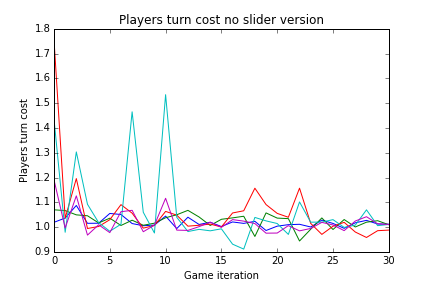
\includegraphics[width=80mm]{images/no_slider_players_costs}
  \caption{Player normalized cost for no slider version.}
  \label{fig:cost_no_slider}
\end{figure}


\begin{figure}
  \centering
  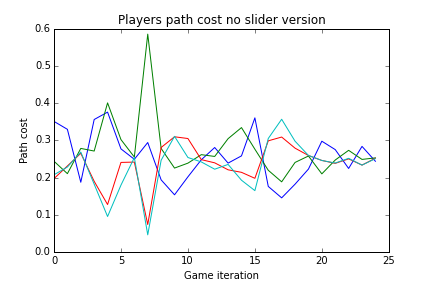
\includegraphics[width=80mm]{images/no_slider_path_costs.png}
  \caption{Predicted path cost.}
  \label{fig:predicted_path_cost}
\end{figure}


\begin{figure}
  \centering
  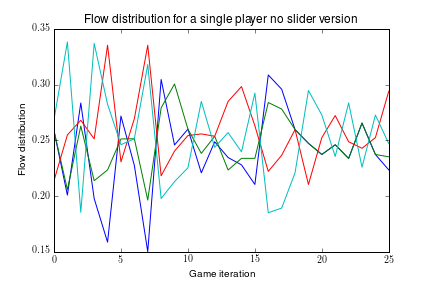
\includegraphics[width=80mm]{images/no_slider_actual_flow_distribution.png}
  \caption{Player flow distribution.}
  \label{fig:no_slider_player_flow_distribution}
\end{figure}

We estimate the learning rate, $\hat \eta^k_t$,  of the players at turn $t$ by

\[
  \hat \eta^k_t = \arg\min_{\eta \geq 0} D_{\psi_k}(\hat x_k^{(t+1)}(\eta), x^{(t+1)}_k)
\]


From these estimated learning rate sequence, we then estimate the flow distribution of iteration $t+1$ using $\hat \eta^k_t $ and $x_k^{(t)}$ with \ref{eq:KL_update}.


%-----------------------------------------------------------------------------------------------------------------------------------------------------------------
\subsection{III}

In the second version of the game, each player were only to change a single parameter $\eta$. This parameter controls how much each player want to explore from their previous flow distribution according to

\begin{equation} \label{eq:KL_update}
  (x_k^{(t+1)})_i = \frac{e^{-\eta_t^k (\ell^{(t)}_k)_i}}{\sum_j (x_k^{(t)})_i e^{-\eta_t^k (\ell^{(t)}_k)_i}}
\end{equation}

From these estimated learning rate sequence, we then estimate the flow distribution of iteration $t+1$ using $\hat \eta^k_t $ and $x_k^{(t)}$ with \ref{eq:KL_update}.

\begin{figure}
  \centering
  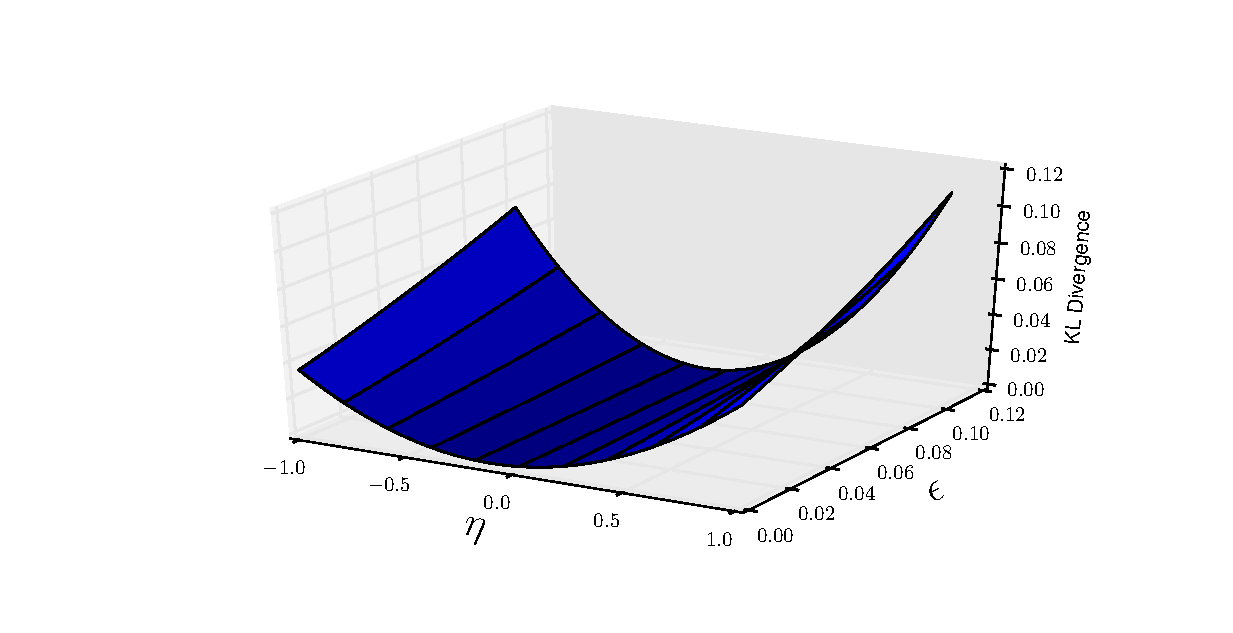
\includegraphics[width=80mm]{images/no_slider_KL_divergence_surface}
  \caption{KL Divergence surface.}
  \label{fig:kl_divergence_surface}
\end{figure}


\begin{figure}
  \centering
  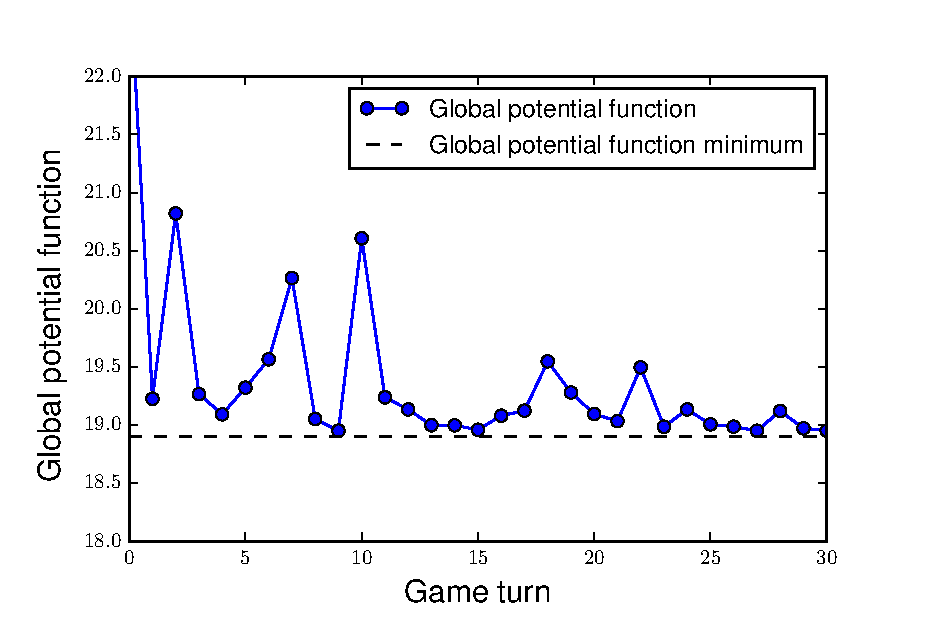
\includegraphics[width=80mm]{images/no_slider_global_potential_function}
  \caption{Global potential function.}
  \label{fig:global_potential_function}
\end{figure}


% \subsection{III}

% In the second version of the game, each player were only to change a single parameter $\eta$. This parameter controls how much each player want to explore from their previous flow distribution according to

% % . The parameter for each turn is shown in \ref{fig:exploration}. We use a small $\epsilon$ to ensure that we will have no underflow for $x_k^{(t)}$ for numerical purposes. Then \ref{eq:KLupdate} becomes

% % \begin{equation} \label{eq:KL_update_epsilon}
% %   (x_k^{(t+1)})_i = \frac{e^{-\eta_t^k (\ell^{(t)}_k)_i}}{\sum_j (x_k^{(t)})_i e^{-\eta_t^k (\ell^{(t)}_k)_i}}
% % \end{equation}


% \begin{figure}
%   \centering
%   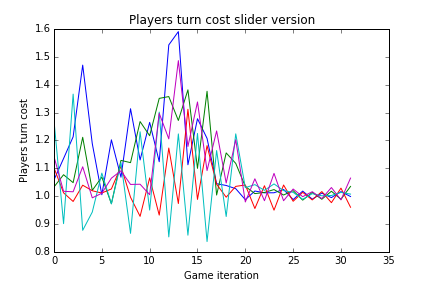
\includegraphics[width=80mm]{images/slider_players_costs.png}
%   \caption{Player normalized cost for slider version.}
%   \label{fig:cost_slider}
% \end{figure}


% \begin{figure}
%   \centering
%   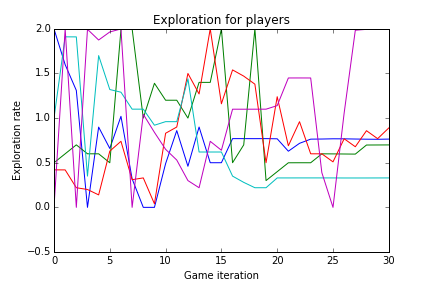
\includegraphics[width=80mm]{images/players_learning_rate.png}
%   \caption{Player exploration rate.}
%   \label{fig:exploration}
% \end{figure}




% \begin{figure}
%   \centering
%   \includegraphics[width=80mm]{images/slider_path_costs.png}
%   \caption{Player exploration rate.}
%   \label{fig:exploration}
% \end{figure}
%-----------------------------------------------------------------------------------------------------------------------------------------------------------------




%============================================================================================
\section{Conclusions}
Conclusion goes here.

%============================================================================================
%ACKNOWLEDGMENTS are optional
\section*{Acknowledgments}
Acknowledgement goes here.

%============================================================================================
%
% The following two commands are all you need in the
% initial runs of your .tex file to
% produce the bibliography for the citations in your paper.
\bibliographystyle{abbrv}
\bibliography{bib}  % sigproc.bib is the name of the Bibliography in this case
% You must have a proper ".bib" file
%  and remember to run:
% latex bibtex latex latex
% to resolve all references
%
% ACM needs 'a single self-contained file'!
%
%APPENDICES are optional
%\balancecolumns
%============================================================================================
\appendix
%Appendix A

Appendix goes here.

% That's all folks!
\end{document}

%%% Local Variables:
%%% mode: latex
%%% TeX-master: t
%%% End:
